\documentclass[conference]{IEEEtran}

% redefine ieee fonts for XeLaTex
\usepackage{etoolbox}
\usepackage{fontspec}
\setmainfont{TeX Gyre Termes}
\setsansfont{TeX Gyre Heros}
\setmonofont{TeX Gyre Cursor}


\usepackage[utf8]{inputenc}
\usepackage{cite}
\usepackage{amsmath,amssymb,amsfonts}
\usepackage{algorithmic}
\usepackage{graphicx}
\usepackage{textcomp}
\usepackage[table]{xcolor}
\usepackage{hyperref}
\usepackage{todonotes}
\usepackage{listings}
\usepackage{bytefield}
\usepackage{xspace}
\usepackage{cleveref}
\usepackage{xspace}
\usepackage{booktabs}

\bibliographystyle{ieeetr}

% Orcid logo for XeLaTeX
\usepackage{academicons}
\definecolor{orcidlogocol}{HTML}{A6CE39}


% more beautiful tables
\rowcolors{2}{white}{gray!25}
\makeatletter
\AtBeginEnvironment{table}{\global\rownum=0\relax}
\def\arraystretch{1.2}
\setlength{\tabcolsep}{2mm}

% enable page numbering, disable for final submission
\pagestyle{plain}

%%% Concepts used in the paper
% Rings
% Interrings
% Envelope
\newcommand{\env}{envelope\xspace}
% System: Inside the Envelope
% Environment: Outside of the Envelope
% Mechanism: A certain mechanism is working as requested by the system
% Mechanism Migration: Making a new mechanism usable by the system
\newcommand{\mm}{Mechanism Interception\xspace}

% Usecase A: TreeTalker Talker
\newcommand{\ttt}{ForestEdge\xspace}
% Useacse B: WireGuard Handovers
\newcommand{\wgh}{TunnelHandovers\xspace}


\begin{document}

%\title{\mm: Modifying Functionality of Communication Systems with Proprietary Components Interceptor }

%\title{Unobtrusive Mechanism Interception: Modifying Functionality of Communication Systems with Proprietary Components }

\title{Unobtrusive Mechanism Interception: \\ 
Teaching an Old Dog New Tricks}

\author{
\IEEEauthorblockN{
    Patrick Lampe\href{https://orcid.org/0000-0002-6233-0959}{\textcolor{orcidlogocol}{\aiOrcid}}, 
    Markus Sommer\href{https://orcid.org/0000-0003-4691-779X}{\textcolor{orcidlogocol}{\aiOrcid}}, 
    Artur Sterz\href{https://orcid.org/0000-0001-9820-7373}{\textcolor{orcidlogocol}{\aiOrcid}}, 
    Jonas Höchst\href{https://orcid.org/0000-0002-7326-2250}{\textcolor{orcidlogocol}{\aiOrcid}}, 
    Christian Uhl, 
    Bernd Freisleben\href{https://orcid.org/0000-0002-7205-8389}{\textcolor{orcidlogocol}{\aiOrcid}}, 
}
\IEEEauthorblockA{
    Department of Mathematics \& Computer Science, University of Marburg, Germany\\
    \{%
        \href{mailto:lampep@informatik.uni-marburg.de}{lampep}, %
        \href{mailto:msommer@informatik.uni-marburg.de}{msommer}, %
        \href{mailto:sterz@informatik.uni-marburg.de}{sterz}, %
        \href{mailto:hoechst@informatik.uni-marburg.de}{hoechst}, %
        \href{mailto:uhlc@informatik.uni-marburg.de}{uhlc}, %
        \href{mailto:freisleb@informatik.uni-marburg.de}{freisleb}%
    \}@informatik.uni-marburg.de
}
}

\maketitle

% In this paper we present e study of mechanism migration and malleable transitions. 
% These two novel approaches open up transitions dedicated for non-transitionable communication systems. 
% First, potential mechanisms suitable for migration are identified, e.g., by methods of static and dynamic software analysis. 
% Methods for the migration of mechanisms are elaborated and selected mechanism migrations are investigated. 
% Specifically, suitable methods for the functional extension of non-transition-capable communication systems by new mechanisms will be explored, such as methods for modification (e.g., binary patching, library preloading, code injection) as well as preemption and redirection (e.g., proxies, splitting of data streams and/or packets). 
% Inherently extensible mechanisms are designed to ensure forward compatibility.
% Deformable transitions are realized exemplarily to gain knowledge about their applicability in real communication systems. 
% From this, recommendations for action and software design patterns for the creation of deformable transitions are derived. 
% Subsequently, the concepts of mechanism migration and deformable transitions are used in combination to realize system-wide cooperative transitions. 
% For this purpose, new mechanisms are introduced into per se non-transition-capable communication systems, which can be deployed by means of automatically adapted deformable transitions under the decision bases given by the target systems. 
% The obtained results are evaluated to demonstrate practical applicability. 
% A systematic evaluation of the performance of selected mechanism migrations and deformable transitions is performed under realistic conditions in the MAKI SDWN testbed (e.g., for web services, applications, smartphones, firmware).


\section{Introduction}
\label{sec:intro}

In our daily life, many devices are used that are based on communication. 
This can be the smartphone, the smart light bulb or the car radio and many other. 
However, computers are not only increasingly used in private life, but also in all conceivable professional areas, for example in industry, computer-supported applications have become indispensable.  
This increased use and the long application of these systems raises the question of how the systems can be supplied with updates over time. 
With open source applications and open source operating systems this may work for experienced users, but for proprietary applications, components or systems this is only possible through the manufacturers.
Especially in the industry where the tasks only computer supported are fulfilled, many devices exist that have this dependence on manufacturers. 
But also in the other mentioned areas proprietary software, components and systems dominate the market.
As long as the manufacturer is willing and able to provide the systems with updates, there is the possibility for the hardware and software components to continue to be supplied with innovations, but if not, then the systems are frozen at this level of functionality. 
Thus, the scope of functionality depends solely on the will of the manufacturer.
Also, new challenges, for example in security, but also in the introduction of new technologies, often lead to the fact that new mechanism is not transferred to all hardware and software components. 
This quickly leads to these systems becoming legacy more quickly than would be necessary. 
By a mechanism, we refer to the concrete implementation of a functional unit that is used by the system to achieve its task. 

In particular, network systems and applications have many protocols that are not proprietary and should be more interchangeable and extensible by design. 
But the protocols used in network systems today have been standardised over a long period of time and implemented in operating systems and devices by the manufacturer.
Much of the internet traffic is based on the TCP protocol \cite{A3:john2007analysis}, which is standardised by the IETF and extended with new parts as needed. 
However, integrating new functionality into existing protocols is very time-consuming and subject to a lengthy process \cite{A3:de2019pluginizing}. 
For example, an approach has been presented in the literature that adds network coding to TCP \cite{A3:sundararajan2011network}. 
These changes are only applicable if the implementation is widely used and both sender and receiver have this extension. 
Another way would be to publish a new protocol with the new functionality instead of extend a existing protocol, but the problem remains the same. 
This creates a fundamental problem: vendor who switch to a new standard or extensions early on have hardly any advantages of their own at the beginning, but without advantages of their own, hardly any vendor will switch.
This means that it takes longer to achieve a certain spread in the market, as a certain critical mass of users must be exceeded. 

But communication protocols are only one level on which this problem occurs, as well as special parts of communication protocols like congestion control or even whole network concepts like DTN or even transmission technologies. 
All these categories have the problem that first enough systems have to be accessible for the functionality to take advantage of the usage. 
This is also true for security mechanisms that should be used for security reasons but are not available in legacy or unmodifiable systems. 
Here, the \mm can contribute to the security of systems by making these security mechanisms available.

In order to achieve the transition capability of networked systems in practice, transitions must therefore be usable on as many devices as possible.
To maximize the benefit for early adopters a method to get new functionality to legacy devices called  \mm seems to be promising.
On the one hand a \mm on the operating-system-level could be a good way to break the innovation blocking point of gaining nearly no benefits for the vendor, by intercepting communication and integrating new functionality to legacy apps and supporting new functionality os wide.
On the other hand the network itself could wrap non-changeable legacy devices to virtually bring new functionality to this devices to support a wide range of them and enable an easy way of bringing new technology much faster to legacy devices and spread new technology. 
In many areas of industry and other businesses, systems such as machines or sensor nodes are in use for many years and are not constantly renewed, especially since this would not be monetarily representable.
In these areas it is essential that new functionality are also made available to these systems.
To address this problem, among others, we introduce \mm. 

% NAT als related Work / als Interceptor
% 6in4 / 4in6
% Wine
% Interceptor Pattern aus Softwaretechnik als Inspiration
% https://patents.google.com/patent/WO2003047205A1/en20
% https://link.springer.com/chapter/10.1007/978-3-030-73885-3_14

% Vergangenheitsperspektive mehr rein bringen
% Die Vergangenheit hat uns nette Dinge gebracht
% NAT 
% Wine 

0Our contributions are:

\begin{itemize}
 \item a
 \item b 
 \item c
\end{itemize}

The paper is organized as follows. 
\section{Related Work}




\paragraph{Inherent extensibility of protocols}
There are various approaches to creating inherent extensibility of protocols.
Foundations for making network protocols extensible and updatable lie in the active networks research branch \cite{A3:tennenhouse1996towards, A3:tennenhouse1997survey}.
ANTS \cite{A3:wetherall1998ants} provides a system architecture that enables new protocols to be deployed on routers as well as terminals through platform-independent code.
Furthermore, a mechanism was presented in the literature that allows new transport protocols to be deployed easily and quickly \cite{A3:patel2003upgrading}. The protocols are exchanged between two communication partners, selected at the beginning of a connection and executed in the kernel.
An additional obstacle in the dissemination of new protocols lies in their use by applications. 
For example, Pathak et al. \cite{A3:pathak2015modnet} present a system that provides applications with additional TCP interfaces and makes TCP adaptable in a fine-grained way, but has hardly been used by applications so far.
With software-defined networks \cite{A3:mckeown2008openflow} and the network programming language P4 \cite{A3:bosshart2014p4}, network programmability was achieved. 
In particular, in the approaches described, the network devices used by providers and service providers become extensible.
Tran et al.~\cite{A3:tran2019beyond} present a method to add functionality to TCP kernel implementation using eBPF. 
As examples, the subsequent implementation of the user timeout option, as well as the dynamic change of the TCP congestion control mechanism are investigated.
QUIC is an alternative to TCP brought forth first by Google and then by the IETF, but is intended to be advanced in a similar manner to TCP.
De Coninck et al.~\cite{A3:de2019pluginizing,A3:de2018tuning} present a method to dynamically tune QUIC on a per-connection basis through extensions. In order to make the QUIC extensions platform-independent, they are executed in a virtual machine.
The presented approaches can be used by actively adapting existing systems and then enable the extensibility of these systems.


In summary, the current state of research still lacks strategies that provide for the inherent extensibility of new protocols and mechanisms -- even for domains where continuous evolution has been shown to occur in recent years. In addition, proprietary system components make it difficult to easily exchange mechanisms on common end devices. Subproject A3 aims to introduce new mechanisms into previously non-transitionable communication systems, thus enabling long-term evolution of communication systslackems.


\paragraph{Network protocols in userspace}
Network stacks are usually implemented in the operating system kernel for efficiency reasons, and existing applications use this kernel implementation. 
To introduce new functionality, it must be implemented in the kernel and adapted to the operating systems in which this functionality is to be supported.
However, network protocols can also be implemented independently of the kernel to allow faster development rates and wider distribution. 
Alpine introduces an alternative network stack in which changes can be implemented and tested quickly \cite{A3:ely2001alpine}.
MultiStack \cite{A3:honda2014rekindling} is a userspace implementation of a network stack framework that can provide isolated network stacks for different applications and enables rapid extensibility. 
An implementation of TCP in userspace is presented by Jeong et al \cite{A3:jeong2014mtcp}.
By executing in multiple threads, it is possible to achieve orders of magnitude higher bandwidth on multi-core machines, but only after the application has been adapted to the implementation.
With NUSE, the network stack of the Linux kernel can be used and further developed as a userspace library \cite{A3:tazaki2015library}. 
Existing programs can thus use modified protocols without modifications to the program itself.
Heuschkel et al.~\cite{A3:heuschkel2016virtualstack} present VirtualStack, which allows different userspace network stacks to be used on one system. 
In these network stacks, extensions as well as new protocols can be implemented and used quickly, and applications can benefit from the protocol changes in the virtual stack without adjustments. 
Especially in cloud applications, decoupling the network stack from the operating system can lead to better adaptability~\cite{A3:niu2017network}.
ClickNF \cite{A3:gallo2018clicknf} is an extension of a software-defined router in which the lower four layers of the network stack can be exchanged in a modular way. 
Extensions of existing protocols, such as TCP, can thus be implemented quickly and easily.
In order to adapt network protocols and the network stack, a system has been presented in the literature with the help of which the network stack can be detached from virtual machines (VM) and centrally managed on the host operating system and made available to the various VMs \cite{A3:niu2019netkernel}. 
SocksDirect \cite{A3:li2019socksdirect} offers the possibility for efficient socket-based communication via local networks. 
Here, a socket system was developed that is completely compatible with Linux sockets and can thus be used for them. 
This requires remote direct memory access between the communication partners in each case. 
The network stack of the operating system is replaced by its own user space implementation without having to adapt the applications. 
Furthermore, a method has been presented in the literature with which energy can be saved on smartphones by shifting parts of the processing of the network stack from the terminals to wireless base stations.
This can save cycles of CPU calculations and thus energy \cite{A3:zhu2016trimming}. 

In summary, it can be stated that despite a high number of related approaches for processing network protocols in user space, the corresponding solutions have not made broad inroads into existing communication systems. There, optimised kernel implementations of the protocols continue to dominate, which are difficult to modify adaptively. Sub-project A3 aims to demonstrate the feasibility of system modifications beyond the user space in principle and to do this, work with pre-positioning of functions and modifications of system components at runtime.



\paragraph{Software-defined wireless networks and modification of wireless communication in existing terminals}
The paradigm of software-defined radio (SDR) promises the highest flexibility in the modification of wireless communication, but to date it is predominantly limited to development platforms and is virtually unheard of in current end devices. Comparably, the approach of Cognitive Radio (CR) considers extensive reconfiguration possibilities of wireless communication with the focus on flexible spectrum use, but also requires specialised end devices. The complete functionality of SDR and CR on terminal systems would be a desirable building block for future, widely programmable communication systems. Today's reality, however, shows that commercially available terminals do not provide for corresponding modification possibilities. 

In recent years, more work on software-defined networks \cite{A3:Kreutz:2015, A3:Monsanto2013} has also been conceived beyond the programmability of the core wired network and extended to wireless communication systems \cite{A3:Bernados:WirelessCommunication, A3:Jagadeesan:2014}. Application-driven SDN-based approaches such as PANE (Participatory Networking) \cite{A3:Ferguson2013}, which served as a model for A3's work in Phase 2, assume that the end devices are completely modifiable. Qadir et al. \cite{A3:Qadir2014} give an overview of programmable wireless networks. Solutions related to subproject A3 in this area include OpenRadio (for configuring various wireless parameters) and OpenRF (for advanced MIMO signal processing with WLAN cards), in which a modification of existing terminal components was made for specialised tasks.
In Phase 2 of MAKI, corresponding work was generalised \cite{A3:ScWeHo2018, A3:GrScLiHo2019, A3:ScLiGrHo2018,A3:MaClScHo2019}, enabling programmability of wireless terminals at the lower layers.

In summary, there is so far only isolated work in wireless communication systems that -- starting from commercially available terminals -- allows a far-reaching modification of the lower network layers. Subproject A3 plans to continue the work started in Phase 2 and to enable far-reaching programmability of the lower layers in terminals as well. This will make it possible to open up non-transition-capable terminals for transitions and thus, for example, to make them capable of meeting mission-critical requirements. 



In Phase 3 of A3, the achievements of the previous phases are taken up.
Work from the areas of data-driven acquisition and adaptation of network properties, as well as participatory decision-making, will be used to construct deformable transitions. 
Nexmon and InternalBlue enabled firmware modifications for wireless network communications, laying a foundation for mechanism migration in firmware.
Inherently extensible protocols as well as user-level networking stacks represent approaches outside of MAKI and are preliminary work that will be used to achieve the goals of Phase 3. 
Taking into account the work presented, a novel methodology is created in A3 to achieve non-transitionable communication systems transition capability using mechanism migration and to deploy malleable transitions under the given framework.

\section{Design}
\label{sec:design}

Networked systems as used today consist of many hardware and software components that are connected to each other to achieve their intended task.
Hosts in a network use gateways to communicate with hosts in other networks, user space applications use system calls to interact with the operating system and hardware components use interfaces to achieve interaction between each other, such as PCI.
However, many of the components can not be updated or upgraded, either due to their proprietary nature or due to lengthy standardization and deployment processes.
This hinders the development of novel applications or improvements of existing systems.
However, developers and engineers already found a way to overcome this problem, by utilizing the environment of such systems and force it behave as desired.

\subsection{Unobtrusive Mechanism Migration by Example}
To illustrate this idea, two examples will be given.

\subsubsection{Network Address Translation}
The Internet Protocol version 4 (IPv4) was designed in the late 1970s and deployed throughout the 1980s.
At that time, the number of participating hosts in the Internet was rather low with less than 1000 and the designers of IPv4 did not anticipate, that the number of hosts in the Internet would increase dramatically as it did especially since the 2000s.
Thus, they chose a 32 Bit field for addressing, allowing only roughly 4.3 billion hosts in the Internet.
With over 5.5 billion devices~\cite{eriscsson2021report}, there are even more smartphones already available globally, not to mention servers, wearables, embedded systems and the entire IoT area.
This development raised the need for solutions.
Althouth there is a newer version of the IP, IPv6 allowing $2^128$ ho

Das erste Beispiel: NAT
Problem, das NAT lösen soll: IPv4 Adressen gibt es zu wenige. Das Ausrollen neuer, besseren Standards dauern jedoch lange, müssen parallel betrieben werden
Sytem: Host, der über das Internet kommunizieren möchte
Environment: Netzwerkzugang
Interceptor: Softwarekomponente auf dem Gateway, der das masquerading anbietet.
Alter mechansimus: routing auf dem Gateway
Neuer Mechanismus: routing wird druch hinzugefügtes masquerading ersetzt
Hinweis: dieses beispiel sollte etwas ausführlicher dargestellt werden, also was wird konkret intercepted, wie findet die Übersetzung statt.

\paragraph{Example 2: WINE}
Zweites Beispiel: Wine
Problem: Ausführung von Programmen auf Betriebssystemen mit inkompatiblen Schnittstellen und Bibliotheken; eine spezifische Implementierung in eimem Anderen Betriebssytem würde das Problem nur für das spezifische System lösen, wine löst es generell durch das Interceptor patter.
System: Programm
Environment: Betriebssytem
Interceptor: Sammlung an überschriebenen Sytemaufrufen und Bibliotheken, Wine
Alter mechanismus: Nutzung der vom betriebyssytem bereitgestellten systemafurufe und bibliotheken
neue Mechanismus: Nutzung von POSIX schnittstellen über hinzugefügte systemafurufe und bibliotheken
Hinweis: auch dieses Beispiel ausführlicher Beschreiben

Die Informatik ist voll von solchen Abstraktionen, etwas <hier zwei weitere Beispiele einsetzen>.
Das ist nicht nur eine Anomalie oder Ausnahme von Funktionserweiterung.
Wie posulieren, dass dieses Vorhegen System hat, sodass wir eine Abstraktion definieren.


\subsection{System Model}
\begin{figure}
    \centering
    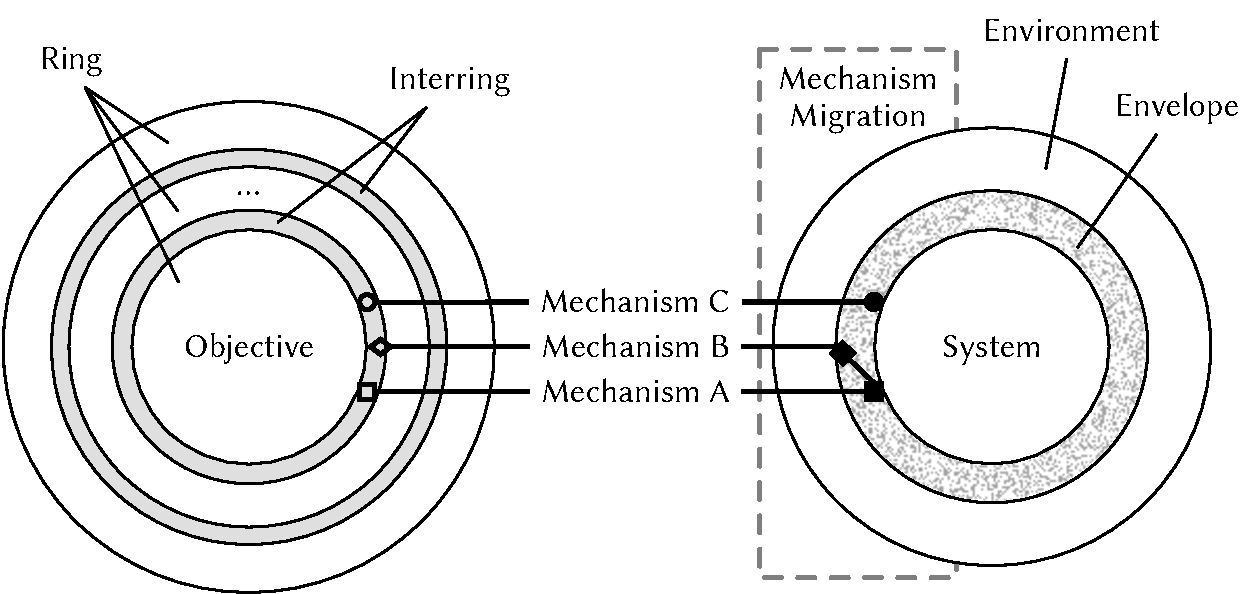
\includegraphics[width=\linewidth]{figures/MechanismMigration.pdf}
    \caption{Mechanism migration to a legacy device with transition-enabled environment}
    \label{fig:bigpicture}
\end{figure}

% Das von uns abgeleitete Modell besteht aus folgenden Komponenten:
The model derived from the above examples and further observations consists of the following components:


\paragraph{System}
At the core of the consideration lies a system that is intended to achieve a specific task.
The system cannot be changed because it is a proprietary component or depends on other external factors, such as high coordination costs for changes due to long standardization or technical hurdles.
This is necessarily so that the system can fulfill its actual task. 
For example, the host in the NAT example needs the routing functionality of the gateway to enable communication with hosts in other networks.

\paragraph{Environment}
Every system is surrounded by an environment that provides functionality for use.
The system has a dependency relationship with the environment, as the system is dependent on the functions provided.
This is necessarily so that the system can fulfill its actual task. For example, the host in the NAT example needs the routing functionality of the gateway to enable communication with hosts in other networks.

\paragraph{Mechanism}
By a mechanism, we refer to the concrete implementation of a functional unit of the environment that is used by the system to achieve its task.
% By a mechanism, we refer to ''a confined conceptual element of a (networked) system that is bound to a realization as cooperating functional units''~\cite{frommgen2016mechanism}.
Mechanisms are located at various points of hardware/software systems, for example:

\begin{itemize}
 \item Complete protocols: TCP, UDP, RTP, overlays, etc.
 \item Specific parts of protocols: congestion control, fragmentation, load balancing, replication, etc.
 \item Network concepts: infrastructure-based, ad-hoc, partially meshed, delay tolerant (DTN), etc.
 \item Network technologies: Ethernet, LTE, IEEE 802.11, Bluetooth, etc.
 \item Security mechanisms: encryption, integrity protection, authentication, etc.
 \item System components: positioning (via WLAN, GSM or GPS), sensors, etc.
 \item Operating System APIs
 \item System Bus Interfaces
\end{itemize}



\paragraph{Interceptor}
In the field of software development, the ``Interceptor architectural pattern allows services to be added transparently to a framework and triggered automatically when certain events occur''~\cite{schmidt2013pattern}.
In this programming pattern, a framework provides interfaces so that programs using this framework can transparently intervene in the flow of data at specific events.

While the goal of our interceptor is basically the same, namely to transparently intervene in the data flow and thus enable new functionalities, the perspective is reversed.
An interceptor in our definition is part of the environment and provides mechanisms to the system via known interfaces. 
In contrast to the interceptor pattern of software engineering, the interceptor is used by the system but configured by the environment so that its use is inevitable.
In order for the system to use the new mechanism, the interceptor is inserted between the system and the mechanism and changes the data flow.
The mechanism to be used can also be introduced into the environment as part of the interceptor and does not have to exist a priori. 


\paragraph{Unobtrusive}
In order not to influence or even disturb the actual task of the system, the mechanism from the interceptor must be unobtrusively replaced by the provided mechanism.
The system must not notice the change of the mechanism, on the contrary the used interfaces must suggest that the original mechanism would be in force.
Furthermore, an interceptor must be unobtrusive so that the system can continue to fulfill the functionality and not provide error cases for the termination.




































%%%%%%%% OLD %%%%%%%%%%%%%
% \begin{figure}
%     \centering
%     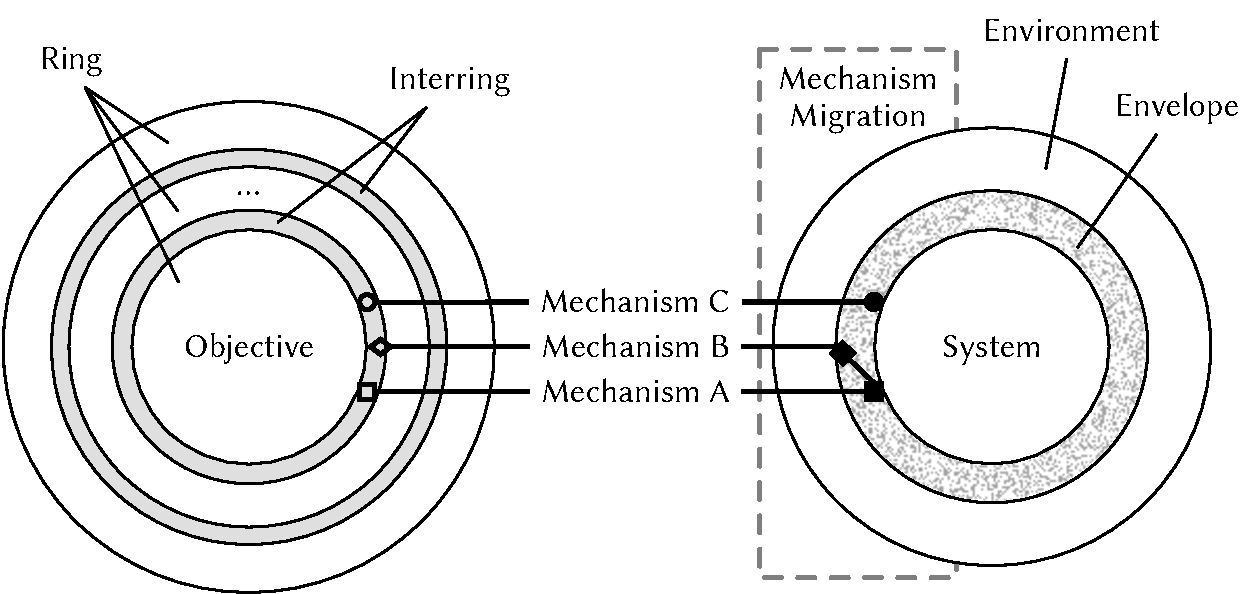
\includegraphics[width=\linewidth]{figures/MechanismMigration.pdf}
%     \caption{Mechanism migration to a legacy device with transition-enabled environment}
%     \label{fig:bigpicture}
% \end{figure}

% The concept of \emph{\mm} allows altering behavior of information and communications system (ICS) that are incapable or unwilling to modify their own operation.
% This could be due to an ICS being built upon proprietary frameworks disallowing modification of the device, manufacturers dropping support or by the unwillingness to make the effort to adapt or update the components of the ICS.
% In such cases developers or network operators are unable to modify the ICS itself.
% However, the proposed approach of \mm enables the modification of an ICS's environment to enforce the desired adaption in its behavior.
% This change can be thought of as an ''outer'' level of the communication infrastructure enveloping an ''inner'' level.

% For example, when faced with a closed application executed on a smartphone, operating system (OS) might be modified to force the applications behavior to change by modifying the OS network stack to transparently wrap connection in a VPN.
% If a whole device is unmodifiable, but the network is under control of the network operator the network can be utilized to force the device to behave in a desired way, e.g. by placing gateway-servers inside the network who can transparently alter traffic flows.
% If even the network is outside control modifying or replacing the communication partner/backend with which the device is communicating is possible.


% \subsection{Rings}
% As the above examples suggest, modern information and communications technology consists of a multitude of components like access devices (smartphones, computers, etc.) and network infrastructure (routers, back-bone network), software (e.g., OSs, middle-ware, applications), networks, network topologies, network protocols on various layers, compute facilities (cloud, edge, etc.) and so on.
% We subdivide these components into a ring structure, as shown in \Cref{fig:bigpicture}, where each \emph{ring} represents a component required for the given domain.
% The most specific component, whose functionality is to be improved by the proposed \mm, forms the center of the structure, called \emph{objective}, while other components are added as rings.
% As an example, an ICS providing a VoIP service to users, the telephony application installed on the end-users device would form the objective, as it should be modified in some way.
% This application requires the OS and its networking APIs, which forms the ring around the application, whereas the next outer ring forms the local area network.
% This categorization allows arbitrary deep rings that seem appropriate for the given domain.
% In the above example, the outer most ring would be the backend executed on a server in the cloud.
% For enabling \mm, it is important to be able to modify or alter rings around the objective, although it is not required to have control of all rings but only the ring required to achieve the desired result.


% \subsection{Interrings}
% Between adjacent rings, components require interaction.
% Such an interface can be anything from set of rules governing the actual communication, such as protocols defined on the different layers of the network-stack-model, to implicit assumptions over the inner workings of peers in a network.
% In the above example, the telephony application uses the OS's networking API to send and receive data.
% Thereon, the OS uses for example Wi-Fi or cellular connectivity to access the local area network, and so on.
% These interaction layers are called \emph{interrings} and are represented as gray layers between the rings in \Cref{fig:bigpicture}.
% Beyond the network stack on a local device itself, interrings include any functionality that allows interaction between two rings like system calls in an application-OS relation or communications between multiple nodes in a network.


% \subsection{Mechanism}
% A \emph{mechanism} is a functional part of an interring that realizes functional units to achieve the desired functionality of the objective.
% Examples of such mechanisms are manifold and span all protocol- and system-layers, as the following selection of possible mechanisms shows:

% \begin{itemize}
%  \item Complete protocols: TCP, UDP, RTP, overlays, etc.
%  \item Specific parts of protocols: congestion control, fragmentation, load balancing, replication, etc.
%  \item Network concepts: infrastructure-based, ad-hoc, partially meshed, delay tolerant (DTN), etc.
%  \item Network technologies: Ethernet, LTE, IEEE 802.11, Bluetooth, etc.
%  \item Security mechanisms: encryption, integrity protection, authentication, etc.
%  \item System components: positioning (via WLAN, GSM or GPS), sensors, etc.
% \end{itemize}

 

% \subsection{Envelope, System and Environment}
% In order to realize the proposed approach, it is necessary to migrate novel functionality to existing ICS.
% An \emph{\env} is a component containing such a new or alternative mechanism that is migrated to the interring between the last ring that is under control and the first ring that is not under control.
% For example, if the telephony application that should support vertical handovers is not modifiable but the OS, the \env containing a mechanism enabling vertical handovers could be placed in the interring between application and the OS.
% It might also be desirable to migrate an \env into an outer interring, although a ring closer to the objective might be still under control.
% All rings, including the objective, that are located within the \env are summarized as the \emph{system} and all rings outside the \env are called \emph{environment}.

 
\section{\ttt}
\label{sec:treetalker}

% For the first case study, we decided to adapt a legacy-device which has been in real-world use for some time.
The \emph{TreeTalker} platform is a product for distributed tree-health monitoring.
This platform has been in use in many areas in the world for example in Moscow city with 250 TreeTalkers or a cooperation with the Peking University\footnote{\url{https://www.nature4shop.com/our-vision/}}.

The platform cosists of sensor-devices (henceforth simply called \textit{TreeTalker}), as well as a base station (henceforth called \textit{TTCloud}), which can be used to relay data via LoRa and upload it to a proprietary cloud-storage provider via GSM.
The TreeTalker-platform is proprietary, and does not give buyers access to the device firmware.
For our project, we aimed to replace the static \textit{TTCloud}, with a more versatile gateway, to allow for dynamic reconfiguration of all \textit{TreeTalkers}.
We call the resulting system \ttt.

The TTCloud, and its associated TreeTalkers, can be configured via text-messages and collected data is sent to the cloud-backend via a mobile data connection using a proprietary call-response protocol, initiated by the TreeTalker.
% \footnote{the operator needs to provide their own SIM-card with a Text-/Data-Plan}
While LoRa-certified hardware provides a dedicated network-layer-protocol, called \textit{LoRa-WAN}, which deals with collisions, addressing, and other issues resulting from the shared-medium characteristic of LoRa, the \textit{TreeTalker}-vendor decided to forgo this higher-level protocol in favor of using the LoRa-PHY-layer directly.
For this reason, communication with each \textit{TreeTalker} needs to be scheduled manually in such a way that avoids collisions.

% In order to replace the \textit{TTCloud} with our own gateway, we performed a blackbox-analysis of \textit{TreeTalker's} behavior and network communications, to understand the communication protocol.

The TTCloud's command message contains 4 types for influencing the TreeTalker's behavior.
\textit{Sleep} is the time that the device will sit idle in between measurements (defaults to 1 hour).
\textit{Heating Time}, that is how long the TreeTalker will run its internal heater before taking the second set of heat-probe measurements.
Lastly, we have the \textit{time slot} and \textit{slot length}.
These values govern the time that the device will wait between measurements and sending measurement data, it appears that these two values are simply multiplied to get the time-to-wait before transmitting.

In normal operation with a vendor-supplied gateway, the sleep- and heat-time are user-configurable, but fixed, and the same for all TreeTalkers attached to the gateway.
The time slot length will also be the same for all nodes, while the gateway will assign each TreeTalker a unique time slot as a result of using LoRa and not LoRa-WAN.
% Again, this is necessary due to the vendor's refusal to use the LoRaWAN-protocol, which includes a mechanism for collision-avoidance, but since the TreeTalker-system uses the raw \textit{LoRaPHY}-layer, the gateway needs to schedule transmission manually.
% For this reason, there is also no way for a TreeTalker-network to coexist with other LoRa-networks in the same area, since collisions would be plenty and unrecoverable.
Finally, the system has no interactivity.
The only way for a user to interact with the system is by downloading a CSV-file containing the measurement data from the vendor's web server.

With the insights gathered by our analysis we were able to fully replace and improve the gateway functionality, which allowed us to bring \mm to the TreeTalker-network.




\subsection{General Design}
\label{sec:TreeTalker:design}
% System: Alle TreeTalker, Ziel: Daten generieen und sie verfügbar machen
% Environment: LoRa Gateway (normalerweise TTCloud) -> Internet
% Mechanism: Lora 
% Interceptor: TTT + Remote (zusammen ForestEdge)
% Unobtrusive: TreeTalker soll keinen Unterschied zw. TTC und ForestEdge erkennen können

\begin{figure}
    \centering
    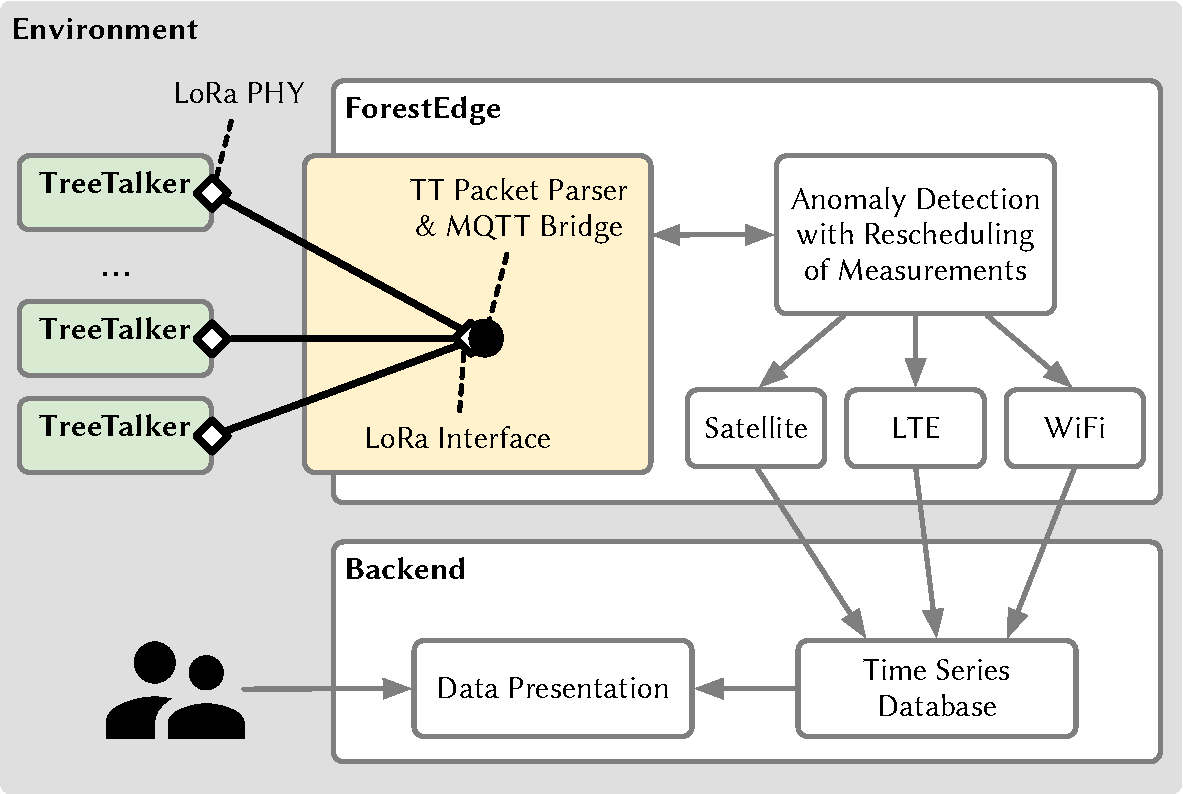
\includegraphics[width=\linewidth]{figures/MechanismInterceptionTTT.pdf}
    \caption{The system architecture for the TreeTalker scenario with interceptor, system and environment as introduced by figure \ref{sec:design}}
    \label{fig:MechanismInterceptionTTT}
\end{figure}

The system in this case study is a swarm of deployed TreeTalkers in a forest,
surrounded by the 
% , its goal is the collection of accurate environmental data and to make it available to users.
b) As for the \textit{environment}, it takes the shape of a forest-wide LoRa network which serves as gateway to connect the TreeTalker swarm to the internet.
It receives the TreeTalker's data via LoRa and can both process it and relay it onwards to other systems on the internet via a variety of mechanisms, such as WiFi, LTE, 5G or satellite uplink.
c) The \textit{mechanism}, which allows the TreeTalker swarm to talk to the system, is LoRa.
d) \textit{\ttt} is the \textit{interceptor}.
It replaces the vendor locked TTCloud, communicates with the TreeTalker swarm via LoRa, and ultimately allows users to access the data in a more convenient format.
Furthermore, it enhances the functionality of the system as a whole by introducing anomaly detection and therefore improve the quality of the collected data.
e) This approach is \textit{unobtrusive}, since the TreeTalkers are unable to distinguish between a first-party TTCloud and \ttt.

Our network architecture employs two separate decision making instances, one is located on the physical device in the forest, which communicates directly with the TreeTalker swarm, and only has data on its directly connected sensors-nodes.
The second, centralized ''aggregator'' instance on the backend, has global knowledge of all nodes in the network.

When the local decision engine receives a packet, it both stores the data locally and also sends it onwards to the global aggregator, which periodically aggregates all the data from all the nodes and computes relevant benchmark values. 
These are then distributed to all stations.
When it generates a reply packet, the local decision engine performs a statistical evaluation on the node's previous measurement data, and how it relates to the aggregator-supplied benchmark values.
If it detects an anomaly, it may require the TreeTalker to rerun its measurements by sending a specially crafted command packet with a short sleep time.

In order to make meaningful decisions, concept recognition is necessary.
This is done by comparing a long-running, and short-running time-window of the data.
It has been shown that the calculation of the twofold standard deviation for short-running windows is already sufficient to be able to make decisions - for example, whether a new measurement is necessary or these new values can be appointed as the new standard.
In general, the preferred decision is to reduce the upcoming measurement interval in order to verify and increase the accuracy of the collected data.
Due to the minor costs on battery and data transmission over Lora, even a 20\% increase in measurements is insignificant for the overall energy consumption. 

\subsection{Evaluation}
\label{sec:TreeTalker:evaluation}

\subsubsection{Response Time}
\label{sec:evaluation:response-time}

The protocol employed by the TreeTalker is a simple two-way exchange of data, where the TreeTalker will send measurements to the associated cloud and wait for new configuration parameters.
If it does not receive a response to its data packet after a certain time, it assumes that the cloud is offline and falls back to repeating the message ad-infinitum.
Thus, in order to be a viable alternative to the first-party TTCloud, the \ttt needs to be able to respond to each received data-packet within reasonable time.

In order to compare the response time of our system versus the TTCloud, we used a test-setup of a single TreeTalker, in combination with a passive sniffing node, which recorded all LoRa-traffic.

\begin{figure}
    \centering
    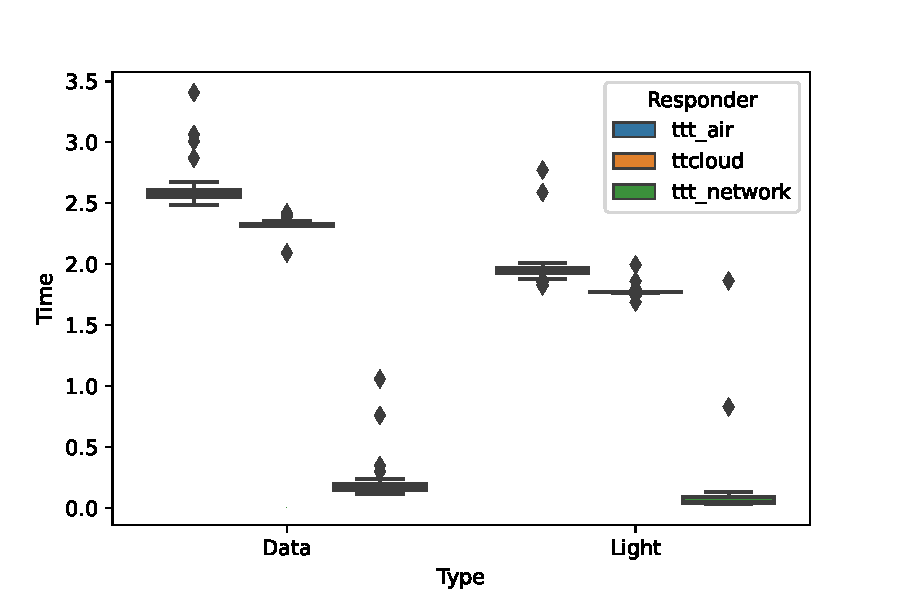
\includegraphics[width=\linewidth]{figures/response_times.pdf}
    \caption{Response time of both the first-party \textit{TTCloud}, as well as \textit{\ttt}.}
    \label{fig:response_times}
\end{figure}

As can be seen in figure \ref{fig:response_times}, the \ttt is capable delivering responses with a similar delay as the TTCloud.
The three bars are, from left to right: 1) The total response time of \ttt, including both the time it takes to generate a reply packet, as well as transmitting it via LoRa. 2) The response time of the first-party TTCloud, also including LoRa Transmission. 3) The time it takes \ttt just to generate the reply packet.
In fact, the actual time it takes to arrive at a decision and craft the reply-package is less than one quarter of the total time, the other three quarters being the time necessary to transmit the packet via LoRa.
The TTCloud, which does no further processing whatsoever, does have the advantage of only sending the same reply every time, thus not requireing any additional time for computations of any kind.
Therefore, it is sometime very slightly faster, though not by any significant margin.

While there are occasional outliers, wherein the analysis of a packet and the generation of the appropriate response packet take significantly longer, these are very rare, being 4 out of 200 cases.
This is most likely due to database-queries occasionally taking longer, probably due to scheduling issues.

\subsubsection{Anomaly Detection}
\label{sec:evaluation:anomaly-detection}

To evaluate whether the anomaly-detection functions as intended, we drew upon real-world data gathered by a TreeTalker-deployment, which was created as part of the \textit{Nature 4.0} project of the University of Marburg.
This deployment is comprised of 100 TreeTalker which were set up in a university-owned parcel of forest and has been continually gathering sensor data for the past 2 years.

The evaluation was performed by injecting historical data into the policy-engine in chronological order, thus simulating a replay of the 2 year data-gathering-process.

\begin{table}[tb]
    \centering
    \caption{Anomalous and critical events found in historical data}
    \label{tab:evaluation:anomalies}
    \begin{tabular}{lcccc}
        \toprule
        Type & Position & Movement & Stem Temp. & Air Temp.  \\ \midrule
        Anomalous & 2182 & 108 & 443 & 0 \\
        Critical & 6313 & 105 & 183 & 1 \\
        \bottomrule
    \end{tabular}
\end{table}

As becomes obvious from table \ref{tab:evaluation:anomalies}, the vast majority of events are produced by the accelerometer, and more specifically by the values denoting the sensor's position.

Further investigation of the data revealed that this seems to be due to a systematical fault in either the installed sensor itself, or the method in which this sensor is queried by the onboard electronics.
The data reported by the TreeTalker for this sensor seems to be completely erratic and entirely unsuited as a basis for further decision-making.
This fault had previously not been noticed by the operator and could have wrought havoc on data analysis performed on the gathered data, but with the aid of \ttt, we were able discover this deficiency before it could impact further decision-making.

\begin{figure}
    \centering
    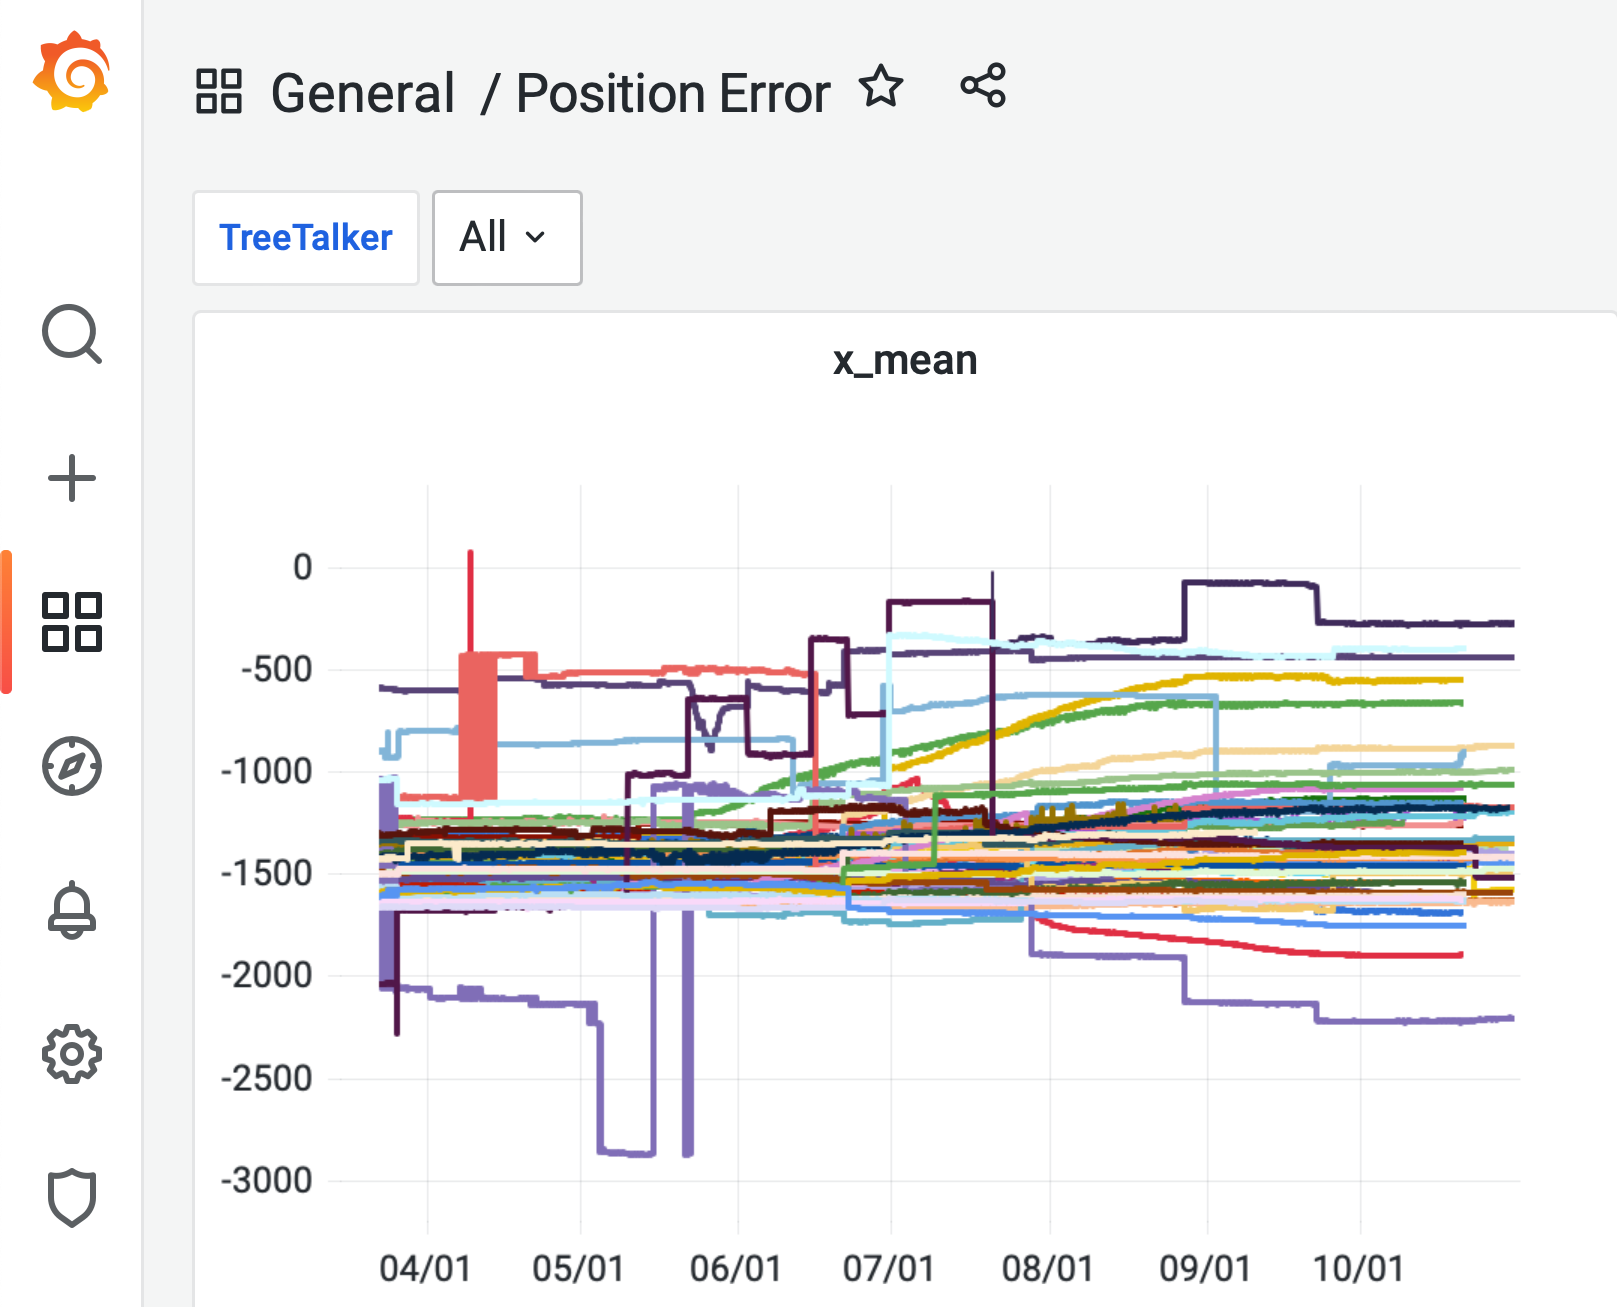
\includegraphics[width=\linewidth]{figures/TTT_position_data_smallest.png}
    \caption{Erratic data from the deployed TreeTalker in the Marburg Open Forest.}
    \label{fig:ttt_position_error}
\end{figure}

In conclusion, by applying our interception-concept to the TreeTalker-network, we were able to significantly improve the system's functionality and performance.
We were also able to leverage behavioral modification to enable interactivity on an otherwise static system, which allowed us to recognize faulty sensors and prevent corrupted data from derailing other research projects.

\newcommand{\ld}{\texttt{LD\_PRELOAD}\xspace}

% klar machen, das doie unobstrusive interception hier das highlight ist, nicht das vertical handover


\section{Vertical Handovers using WireGuard}
\label{sec:wg:impl}

A major unsolved problem in today's mobile communications is vertical handovers.
Vertical handover (simply called handovers from now on) describes the switching process of a networked device from one network access to another.
Probably the best-known example is the switch from Wi-Fi to a cellular connection, for example when leaving home on the way to the office.
The core problem with handover is protocols such as TCP, which were designed in a time when wireless communication did not yet exist and therefore disconnections on the transport layer were not foreseen.
If the connection on the transport layer is interrupted, the connections on the application layer must also be re-established, which can lead to different implications for different applications, such as interruptions of audio streams when listening to music or making phone calls.
Several solutions have already been discussed in the past.
There are standards that explicitly support mobility of nodes and implement mechanisms to support handovers, most notable Multipath-TCP, SCTP and QUIC.
However, all these approaches have the core problem that they have to be deployed and supported by all participants in the network.
So far, none of these protocols have gained any substantial deployment.
Further, all of these solutions require application developers to update and adjust their application to support these protocols, further hindering broad usage.

In this section, we present an approach that uses common Linux mechanisms to enable handovers without TCP session disconnects, and without the need to roll out new, complicated, or niche protocols.


\subsection{General Design}
The approach presented in this section relies on two building blocks: WireGuard and \ld.
WireGuard is a simple, fast and secure VPN software that transmits encrypted data encapsulated in UDP datagrams.
The use of UDP for communication eliminates the problem of TCP connection losses during handovers since neither UDP nor WireGuard is connection-oriented.
% Once an initial handover is complete, WireGuard sends the UDP datagrams over the new connection without the TCP connection tunneled through the WireGuard VPN noticing.
% To realize our approach the WireGuard software needs to be installed on the system, which can either be done as a kernel module or, if no kernel module is available (e.g., for non-Linux based systems or the kernel of the system can not be modified) as a platform-independent user space version.
% For this approach both alternative are possible.
For the WireGuard tunnel to work, an additional tunnel endpoint somewhere in the network is required, at which the WireGuard tunnel is terminated and the encapsulated TCP connection further relayed to the original destination.

The use of WireGuard alone does not automatically enable existing TCP-based applications to support handovers.
Rather, they have to be instructed to transfer their data over the WireGuard connection.
One way to do this, is to modify the routing table of the system in a way, that all traffic from the host is sent over the tunnel.
However, this would mean that non-TCP based applications would also be routed through the tunnel, including UDP or QUIC based applications that do not have the problem of missing handover capability.
% This approach would just add the overhead of WireGuard for these applications without gaining anything.
% This is where \ld comes into play.
To mitigate this potential drawbacks, \ld is used.
The \ld mechanism allows overriding functions of dynamically linked libraries, enabling to override the socket API of Linux such that only connections of the application started with our \ld modifications are using the WireGuard tunnel.

The rough procedure is as follows.
A WireGuard daemon is run on the local system.
When a program is executed with our \ld modifications, the TCP packets of this particular application are passed to the local WireGuard daemon.
The UDP-based WireGuard packets are then sent to the WireGuard endpoint located in the network, which unpacks the encapsulated TCP connection and acts as a relay to forward the application data to the desired destination using conventional TCP/IP mechanisms.
The responses from the server with which the application is communicating are sent back to the host via the same route, i.e. via the WireGuard tunnel.
The exact implementation and configuration will be discussed below.

\subsection{Implementation}
% Several implementations lead to the desired result, but with different drawbacks.
% The first approach would be to configure the WireGuard in a way so that no traffic is sent through the tunnel and the \ld implementation sets a rule in the routing table that causes the traffic of an application to be sent through the WireGuard tunnel on a IP address basis.
% However, this approach has several disadvantages.
% First, three functions of the socket API must be overridden, \texttt{socket}, \texttt{connect} and \texttt{close}.
% The \texttt{socket} system call returns a file descriptor and the \texttt{connect} call connects to a given IP address over the socket with the file descriptor of the previous \texttt{socket} call.
% Once both the file descriptor and the IP address are available, the routing table has to be modified by adding a rule to route the extracted IP address over the WireGuard interface.
% This, however, has the disadvantage that other applications that have the same endpoint would also be tunneled through WireGuard.
% Finally, when the the client closes a connection, the \texttt{close} system call is used.
% the \ld implementation at this point has to remove the rule from the routing table to restore the original state.
% However, to realize this cleanup, a mapping is required between the file descriptor and the corresponding IP address leading to both implementation and runtime overhead for this mapping, as the \texttt{close} system call only closes a file descriptor.

% An alternative approach is to bind a socket to an interface using the \texttt{SO\_BINDTODEVICE} socket option.
% Using this option, the socket is advised to route all traffic that is sent to the given file descriptor using a specific interface, in our case the WireGuard interface.
% This approach has multiple advantages.
% First of all, it only requires the \texttt{socket()} system call to be overridden.
% Whenever the application opens a new TCP socket, our \ld implementation binds this socket to the WireGuard interface.
% Second, it has minimal implementation and runtime overhead, as there is no state that has to be maintained as in the above approach.
% Finally, as soon as the application closes the socket using the \texttt{close()} system call, the binding created by our \ld implementation is also removed by the Linux kernel.
% However, this approach comes with the downside that the Linux kernel has a security mechansism called \textit{Reverse Path Filtering (RPF)}.
% One of our goals is that only connections of applications using the \ld implementation are routed through the WireGuard tunnel.
% To solve this either a route for each application has to be set, which leads to the rejected solution from above.
% Alternatively, a second routing table is created for the WireGuard interface.
% If the application's socket is bound to the WireGuard interface because the application uses our \ld implementation, the Linux kernel will still send and route packets via the interface, since an entry exists for this interface in the second table.
% The problem now is that responses from the server are dropped by Linux because of said RPF.
% When the kernel receives an IP packet, it checks whether the source of the packet is reachable through the interface through which it was received.
% If the packet can be forwarded over the interface from which it came, the computer accepts the packet, otherwise it will be dropped.
% In our case the packet is not routable, because the kernel only looks in the standard routing table, but does not find an entry for the IP address.
% The solution is to use policy based routing to tell the kernel to look in the second routing table for a specific IP address range, namely that of the WireGuard interface.


One of our goals is that only connections of applications using the \ld implementation are routed through the WireGuard tunnel.
Forwarding traffic of a certain TCP socket to WireGuard is implemented using the \texttt{SO\_BINDTODEVICE} socket option.
Using this option, the socket is advised to route all traffic that is sent to the given file descriptor using a specific interface, in our case the WireGuard interface.
However, this approach comes with the downside that the Linux kernel has a security mechanism called \textit{Reverse Path Filtering (RPF)}, which becomes active.
To cope with this problem, a second routing table is created for the WireGuard interface.
If the application's socket is bound to the WireGuard interface, the Linux kernel will still send and route packets via the interface, since an entry exists for this interface in the second table.
In addition, policy based routing is used to tell the kernel to look in the second routing table for a specific IP address range, namely that of the WireGuard interface.
 



\subsection{Experimental Evaluation}
To evaluate the proposed approach and show the feasibility of enabling existing TCP-based applications to perform seamless handovers, we performed extensive emulations in two scenarios.
% In this section, we present the experimental environment and discuss the evaluation results.


\begin{figure*}[tb]
    \centering
    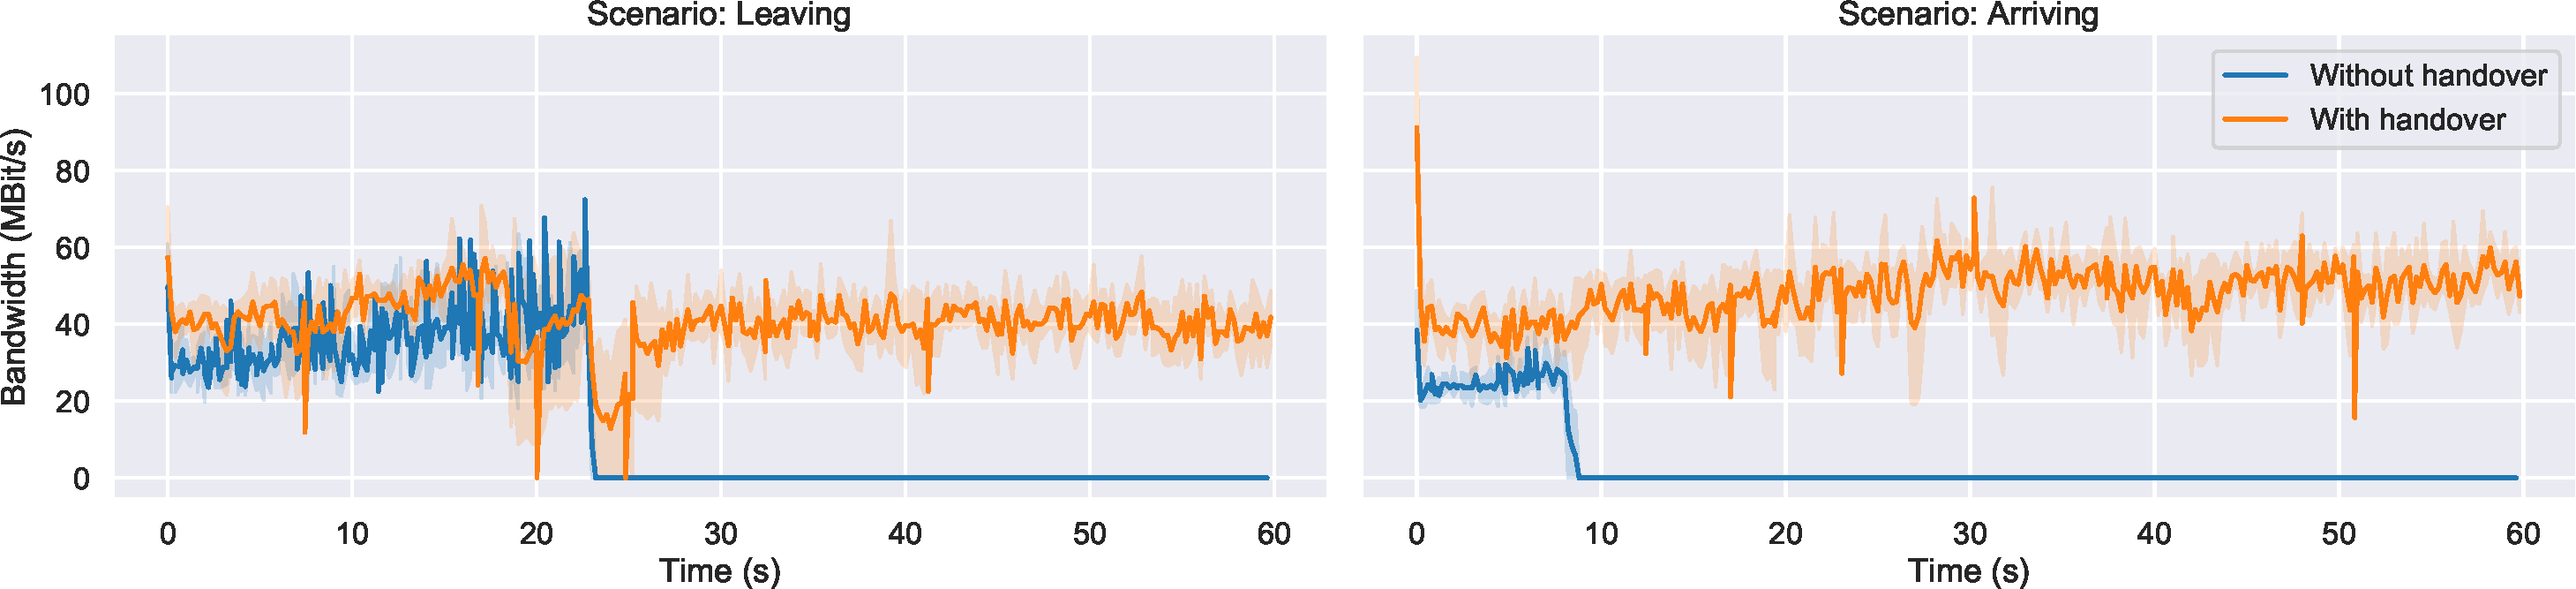
\includegraphics[width=\textwidth]{figures/migration/wg_migration-network.pdf}
    \caption{Network throughput with and without connection migration for two scenarios}
    \label{fig:eval:mig:network}
\end{figure*}
\begin{figure*}[tb]
    \centering
    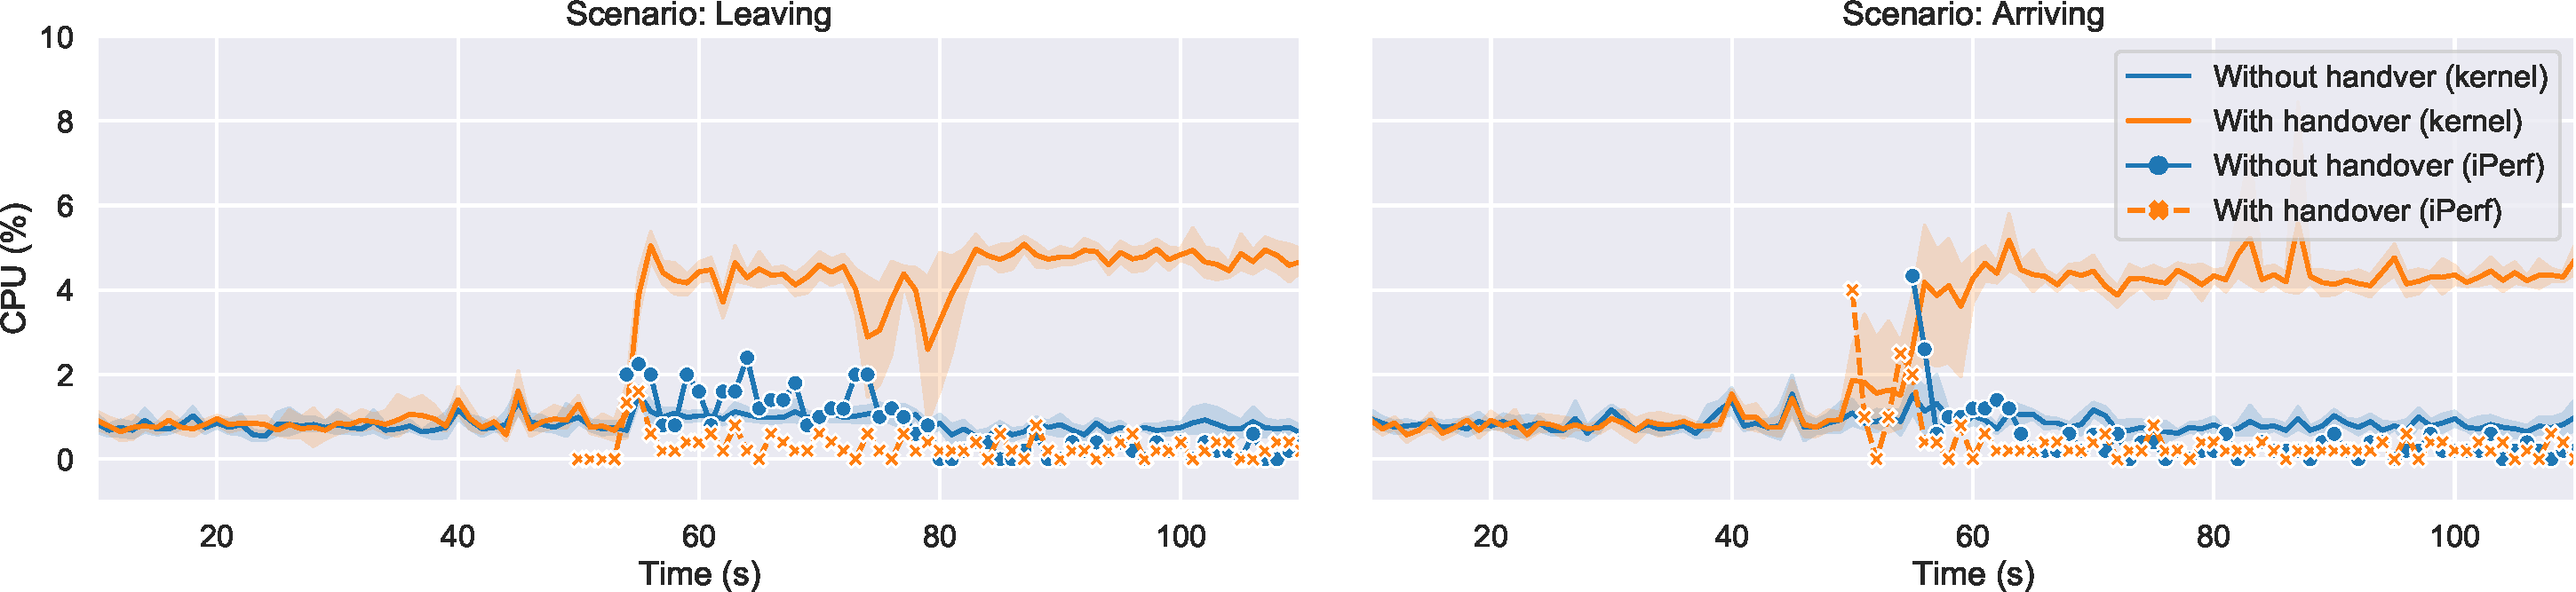
\includegraphics[width=\textwidth]{figures/migration/wg_migration-cpu.pdf}
    \caption{CPU usage with and without connection migration for two scenarios}
    \label{fig:eval:mig:cpu}
\end{figure*}


\subsubsection{Experiment Setup}
% \paragraph{Emulation}
To conduct the evaluation, two scenarios were emulated, of which the first one (S1) simulates leaving a location.
Here, the handover is performed from Wi-Fi to LTE.
The second scenario (S2) simulates the corresponding handover from LTE to Wi-Fi, e.g., when entering a building providing a Wi-Fi connection.
In order to perform these experiments, the \emph{Common Open Research Emulator (CORE)}\footnote{\url{https://coreemu.github.io}} was used, that allows execution of arbitrary programs.

\begin{figure}[ht]
    \centering
    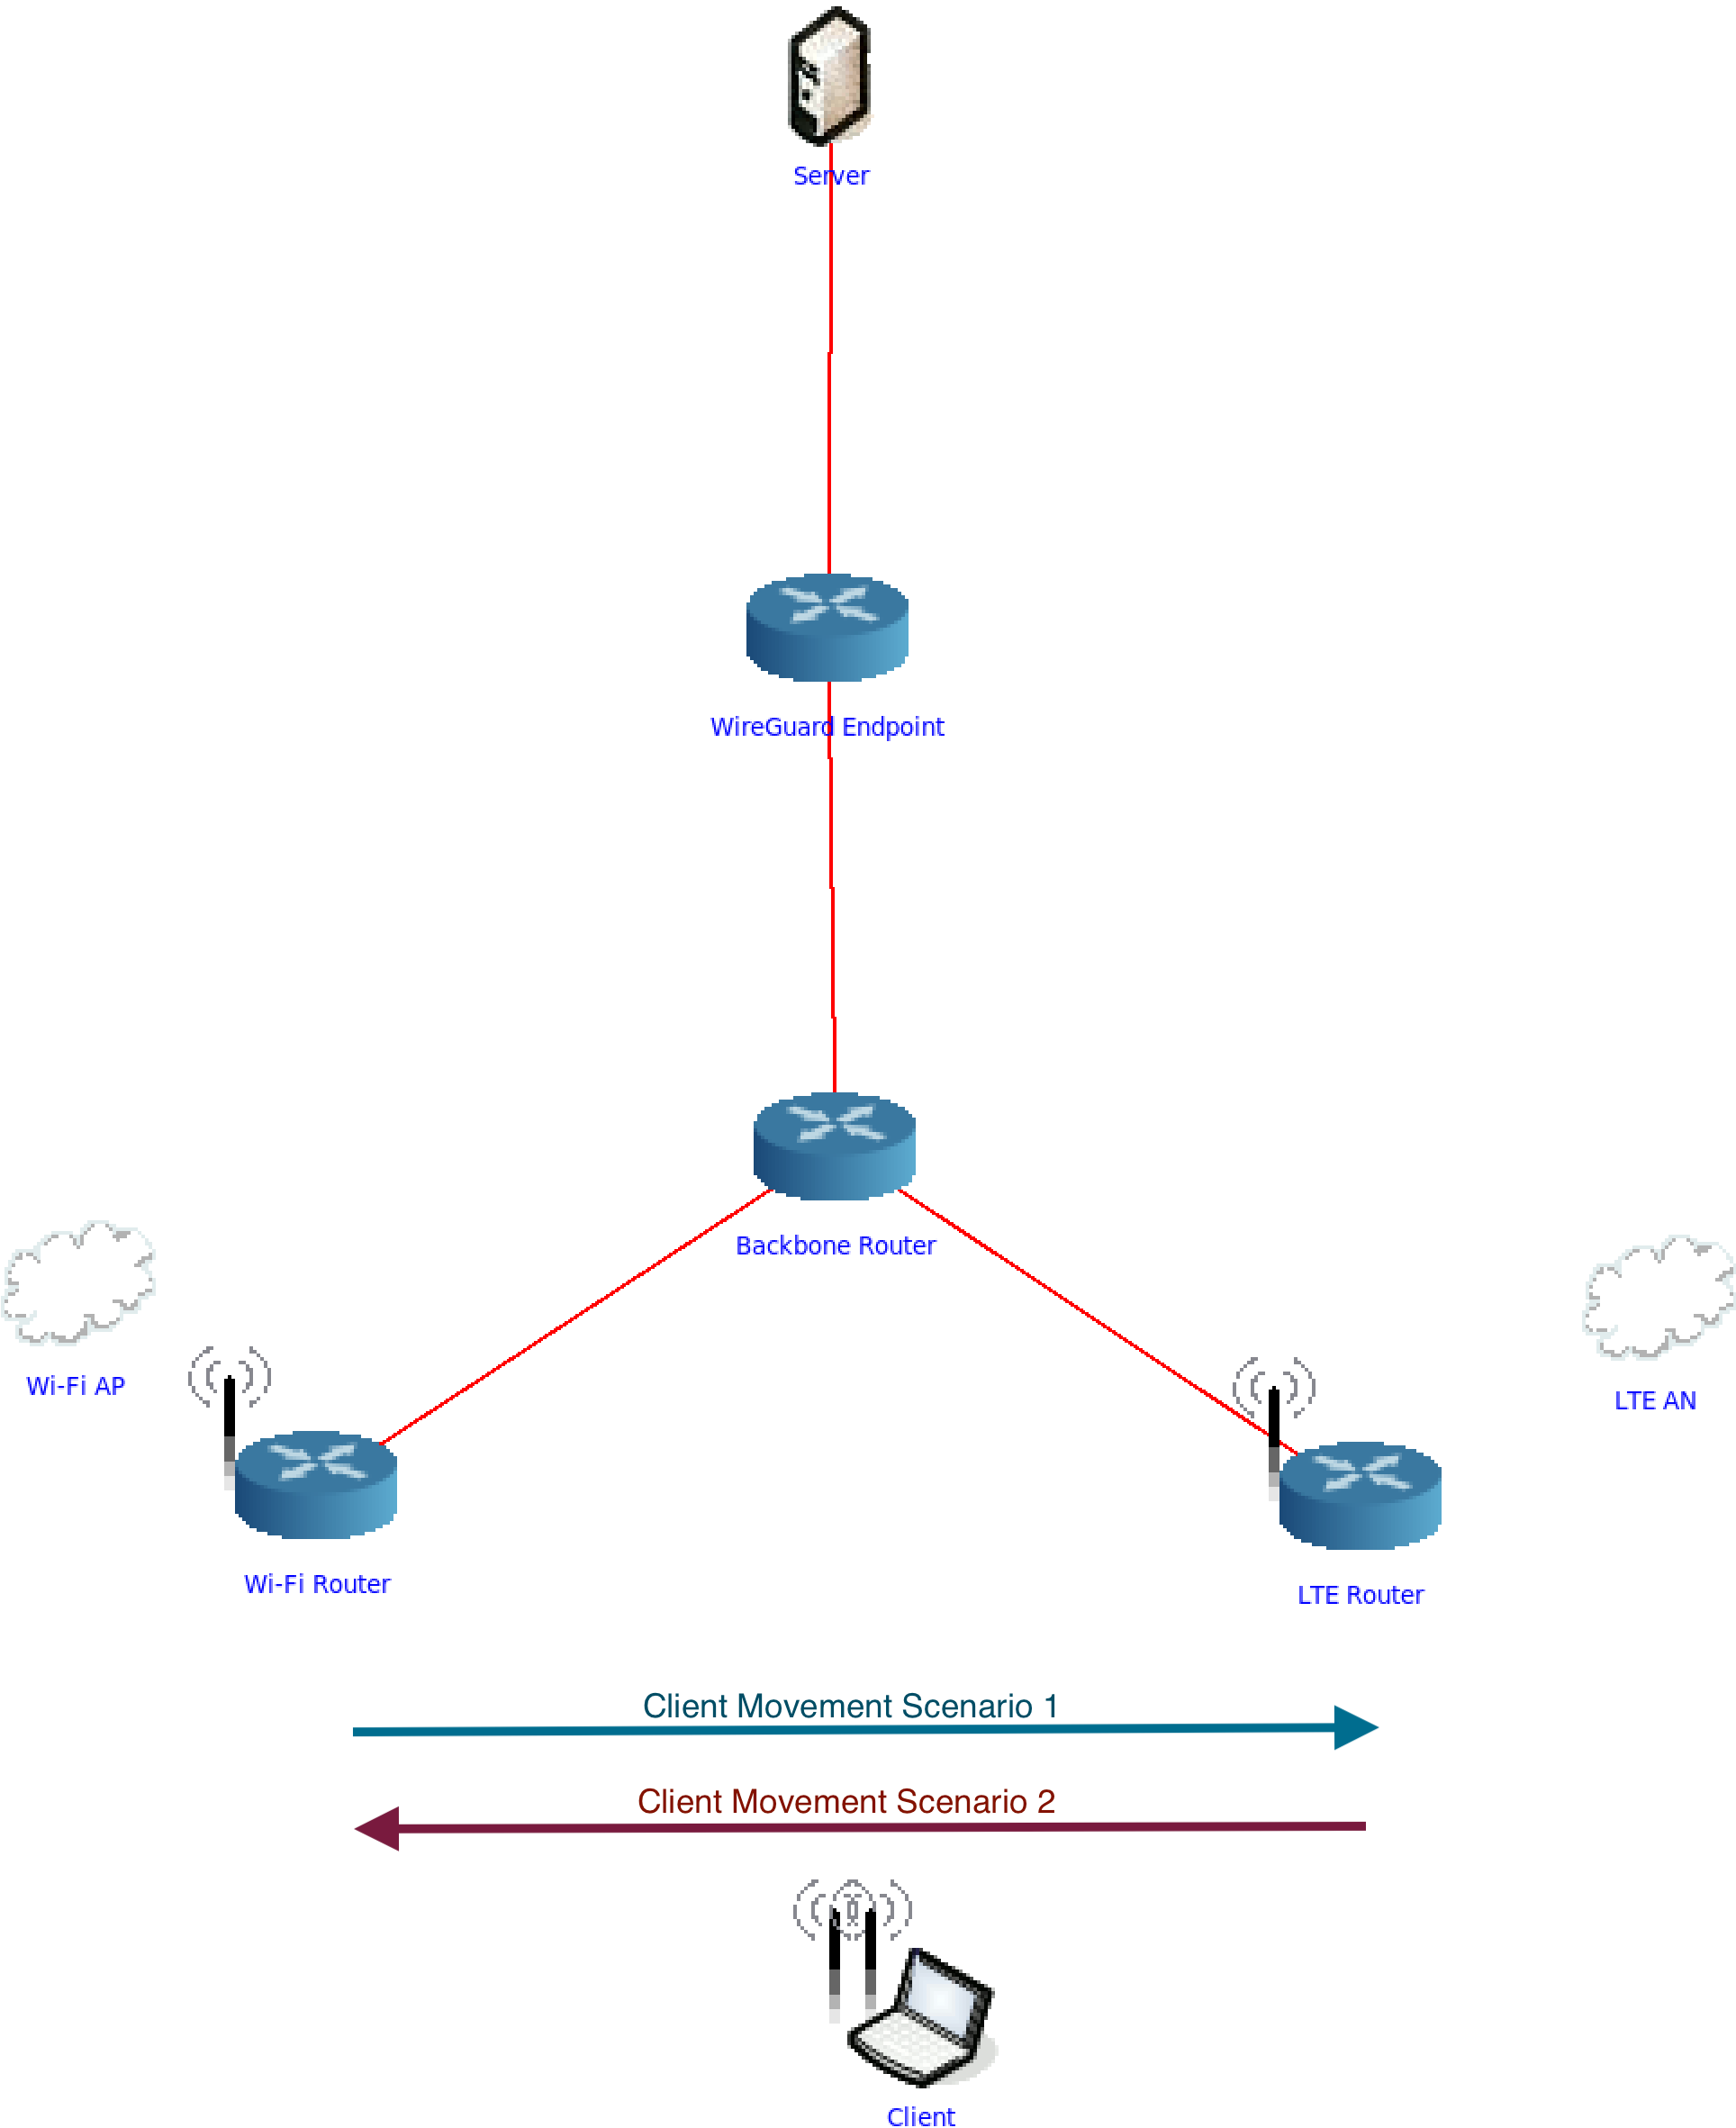
\includegraphics[width=.9\columnwidth]{figures/migration/topo.png}
    \caption{Simulated topology used for the evaluation}
    \label{fig:eval:mig:topo}
\end{figure}

% \paragraph{Topology}
Fig.~\ref{fig:eval:mig:topo} shows the topology used for the evaluation.
% Within the emulation, the following nodes were modeled.
% First, a mobile client node is required, which is the bottom node in Fig.~\ref{fig:eval:mig:topo}.
The client (bottom) contains the TCP-based application that shall be enabled with handover capabilities and the WireGuard client.
Further, the client node is the only node moving throughout the emulation.
In S1, the client moves from left to right (blue arrow) and loses the Wi-Fi connection roughly in the middle of the movement range. 
In S2, the node moves from right to left (red arrow) and regains the Wi-Fi connection at the same position.
The LTE connection is available throughout the entire experiment, whereby the Wi-Fi connection is prioritized if available.
The mobility is modeled in a way to simulate human walking, i.e., 5 to 6 km/h.
Further, we modeled a Wi-Fi access point (Wi-Fi AP on the left) and a corresponding Wi-Fi router.
% The client is connected to the Wi-Fi AP, which in turn uses the Wi-Fi router to route traffic.
We modeled the Wi-Fi AP to match the IEEE 802.11ac standard, i.e., roughly 1 Gbit/s throughput.
On the bottom right in Fig.~\ref{fig:eval:mig:topo}, the LTE access network (LTE AN) was modeled to match current LTE speeds of about 100 MBit/s.
% The LTE AN is connected to a LTE router.
In the middle of the topology, a router was modeled to mimic the backbone of the network, i.e., the network of an ISP connecting multiple parts of the Internet.
The second node from the top is the WireGuard endpoint, that is used to terminate the WireGuard tunnel.
% From this node, the arriving encapsulated TCP connection from the client is extracted and relayed to the server and TCP-packets from the server encapsulated and transmitted using WireGuard to the client.
% The WireGuard endpoint node also acts as a regular backbone router in experiments not using the WireGuard tunnel.
Finally, the server node is modeled (top), which only contains the application's server.

% The red connections in Fig.~\ref{fig:eval:mig:topo} represent wired connections between the corresponding nodes.
% The connection between the Wi-Fi router and the backbone router is modeled to mimic a standard uplink that can be found in homes with 100 MBit/s.
% The other wired connections are using links of multiple GBit/s, which are however not relevant as the limiting links are the LTE AN connection and the connection between the Wi-Fi router and backbone router.

% \paragraph{Applications}
In order to simulate a TCP-based application, iPerf3\footnote{\url{https://iperf.fr}} was used.
iPerf3 is an open-source tool for measuring network throughput in IP network following the client-server paradigm and supports various transport layer protocols.
% The server node in the evaluation topology runs an iPerf3 server, whereas the client node runs the iPerf3 client.
The client initiates the connection to the server upon experiment start using the currently active connection, i.e., Wi-Fi if available, otherwise LTE.
Each experiment was executed for 120 seconds in total.
Within the first 50 seconds, where used to allow the emulation establish routes throughout the network, so that packets can be routed from client to server and back again.
As soon as the routes were announced, the movement and iPerf started for 60 seconds.
The last 10 seconds were used to tear down the emulation.
In addition to the presented handover-approach, we also conducted experiments without a tunnel, using the regular routing mechanisms of the Linux kernel to be able to compare the achievements of our approach.
Each experiment was repeated five times to reduce effects like race conditions during booting the emulation and other side effects.

\subsubsection{Results}

% \paragraph{Supporting Vertical Handovers}
Fig.~\ref{fig:eval:mig:network} shows the results for the conducted experiments.
The x-axis denotes the experiment time, while the y-axis denotes the achieved bandwidth.
The left sub-plot visualizes the leaving scenario, while the right sub-plot visualizes the arriving scenario.
Finally, the orange graphs show experiments, where the proposed handover mechanism is enabled, the blue graphs show the results without employing the WireGuard tunnel for comparison.
As can be seen in both scenarios, the proposed approach for using WireGuard to enable TCP-based applications with vertical handover capabilities, works  as proposed.
Especially in the arriving scenario, the throughput of the iPerf application does not drop at all.
Without the WireGuard tunnel, throughput decreases because the iPerf or, in particular, the TCP connection is not re-established after the connection is changed.
In the leaving scenario, a small drop is visible at around 25 seconds.
This is due to the fact that the Wi-Fi connection is lost immediately, resulting in a short connection drop until he kernel recognizes the lost connection and propagates the changes to the routing tables.
In the arriving scenario, however, this drop is not visible since the LTE connection does not break but rather the Wi-Fi connection is established in parallel.
As soon as the kernel detects the new Wi-Fi connection, the WireGuard tunnel uses the Wi-Fi connection, whereas in the blue graph it is visible, that, although the LTE connection is still available, the TCP connection does not continue due to the newly established Wi-Fi connection.

% \paragraph{Overhead Analysis}
Although the handover capabilities offer a great improvement for users, the WireGuard tunnel introduces some kind of overhead because it has to encapsulate the TCP-connection and introduces encryption.
To quantify this overhead, the CPU usage of both the kernel and the iPerf process was monitored, which can be seen in Fig.~\ref{fig:eval:mig:cpu}.
Fig.~\ref{fig:eval:mig:cpu} is composed the same way as Fig.~\ref{fig:eval:mig:network}.
The y-axis, however, denotes the CPU utilization of the client node.
Further, the solid graphs show the kernel's CPU usage, while the graphs with markers show the CPU utilization of iPerf.
First, the iPerf CPU usage does not differ significantly, regardless of the scenario and whether the WireGuard based handover mechanism is used.
The kernel, however, shows quite a different result.
On the one hand, the blue graphs, i.e., without the WireGuard tunnel, show that the kernel's CPU utilization is relatively constant at around 1\% for the entire experiment.
In the orange graphs, on the other hand, show an increase of CPU utilization of around 3\% as soon as iPerf starts sending data, which is the same for both scenarios.
The two drops in the leaving scenario around the 80 seconds mark align with the network drop visible in Figure~\ref{fig:eval:mig:network}, where iPerf is not able to send data for the time of the handover.

Considering the improvement in the users' connection with consistently high network quality using our method, only 3\% of additional CPU consumption is an acceptable overhead.
Moreover, iPerf specifically tries to make maximum use of the available bandwidth.
For applications that have a normal usage profile, it is to expect that the overhead will be significantly lower.
Finally, the authors have shown in past work how to reliably predict Wi-Fi connection loss~\cite{hochst2019learning}.
Thus, a system that only activates the WireGuard tunnel when a connection loss is expected is conceivable, which would limit the CPU utilization overhead to a few seconds in time.

\section{Conclusion}
\label{sec:conclusion}

We presented \emph{\mm}, a novel approach providing a model to implement unobtrusive functional additions to or modifications of an existing networked system without touching any proprietary components.
By classifying a networked system into the \emph{system}, i.e., components containing proprietary or other not changeable parts, and the \emph{environment}, i.e., components containing modifiable parts under control, 
behavioral changes are achieved by mechanism-enhancing yet unobtrusive \emph{interceptors},
i.e., a layer that is introduced between environment and system adding or updating mechanisms.
Such an interceptor can have many forms like an updated software library, a newly deployed edge device, or an enhanced cloud service.
Interceptors must be unobtrusive to avoid disrupting or even breaking applications but still provide added or modified mechanisms to the networked systems.

We illustrate this approach by applying the findings of the model in two case studies
that show its real-world applicability.
First, we unobtrusively replace a cloud infrastructure by an edge infrastructure in a wireless sensor network.
Second, we unobtrusively add a vertical handover mechanism between Wi-Fi and LTE to a mobile end device without disconnecting TCP sessions.
Our results indicate that \mm is a compelling approach to achieve improved service quality and provide previously unavailable functionality in an unobtrusive manner.

The contributions of this paper are:
\begin{itemize}
    \item We present \mm, a model that can be used by developers to design and implement unobtrusive mechanism interceptors.
    \item We present two examples, NAT and Wine, which serve as a basis for developing the \mm model.
    \item We present an application, \ttt, where our model is applied to replace a cloud infrastructure by an edge infrastructure to unobtrusively add previously unavailable functionality in a sensor network.
    \item We present an application, where our model is applied to add an unobtrusive vertical handover mechanism between Wi-Fi and LTE and thereby improve service quality of mobile devices.
\end{itemize}

The remainder of this paper is organized as follows.
Section~\ref{sec:releted_work} presents related work.
Section~\ref{sec:design} introduces two real-world examples and the derived model for \mm.
Section~\ref{sec:treetalker} presents the first case-study, \ttt and Section~\ref{sec:wg:impl} presents the second case-study, \wgh.
Section~\ref{sec:conclusion} concludes this paper and presents future work.


\section*{Acknowledgments}
This work is funded by the Hessian State Ministry for Higher Education, Research and the Arts (HMWK) (LOEWE Natur 4.0, and LOEWE emergenCITY), the German Academic Exchange Service (DAAD) (Transformation Partnership Program; Project OLIVIA), and the German Research Foundation (DFG, Project 210487104 - Collaborative Research Center SFB 1053 MAKI).


\bibliography{main}
\end{document}